	\begin{figure}[t]
		\label{fig:comparison}
		\centering
		\subfigure[We propose a novel approach for propagation as well as training.]
		{
			\begin{minipage}{0.65\textwidth}
				\centering
				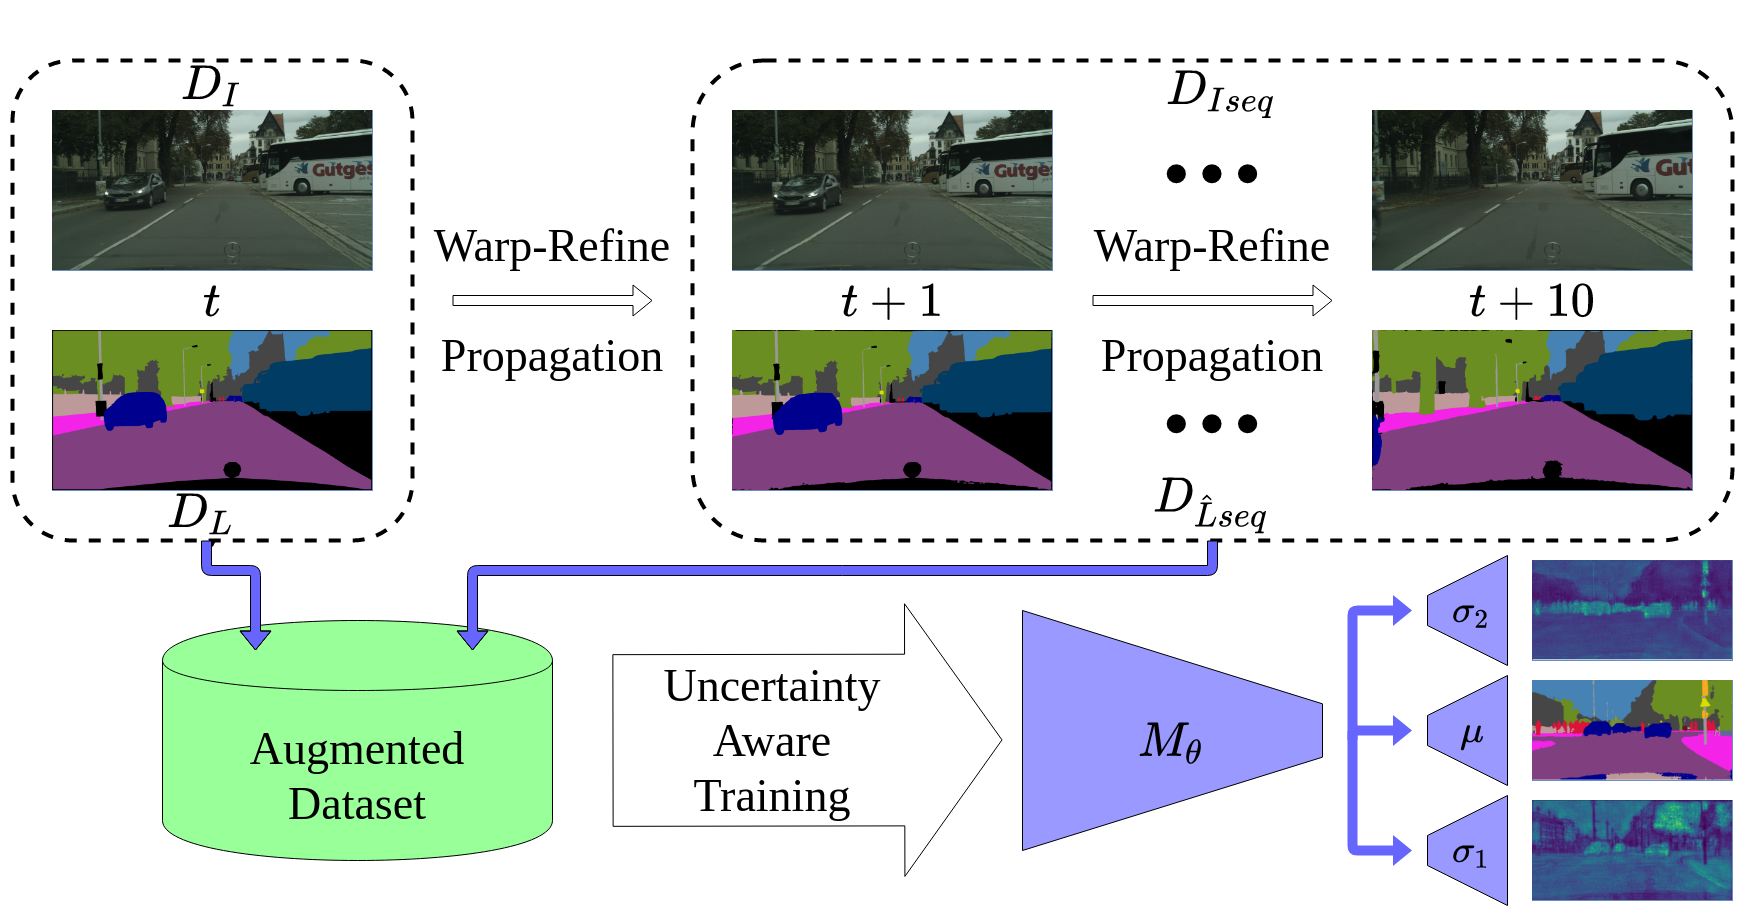
\includegraphics[width=1.0\linewidth]{figures/overview_lr.png}
				\vfill
			\end{minipage}
		}
		\hfill
        \hspace{-2em}
		\subfigure[Top:~\cite{nvidia_cvpr19}, Bottom: Ours]
		{
            % \begin{minipage}[b][0.315\textheight][s]{0.315\textwidth}
            \begin{minipage}{0.33\textwidth}
% \subfloat[(a)]{%
%   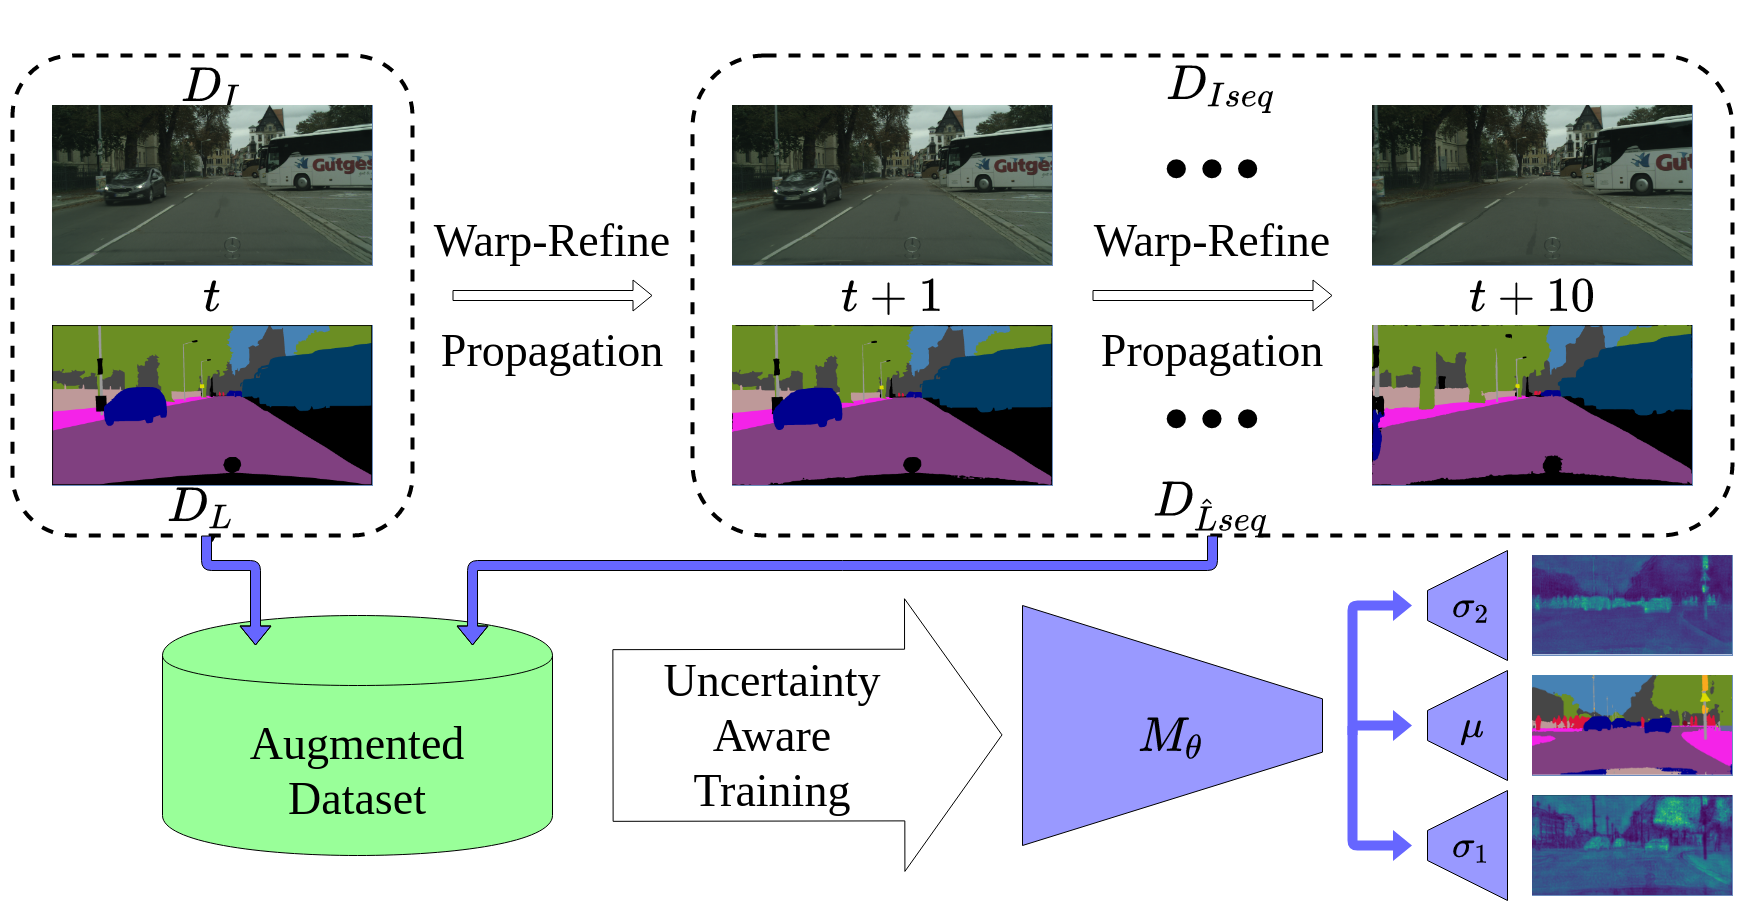
\includegraphics[clip,width=0.315\textwidth]{figures/fig_overview_lowres.png}%
% }
% \subfloat[(b)]{%
%   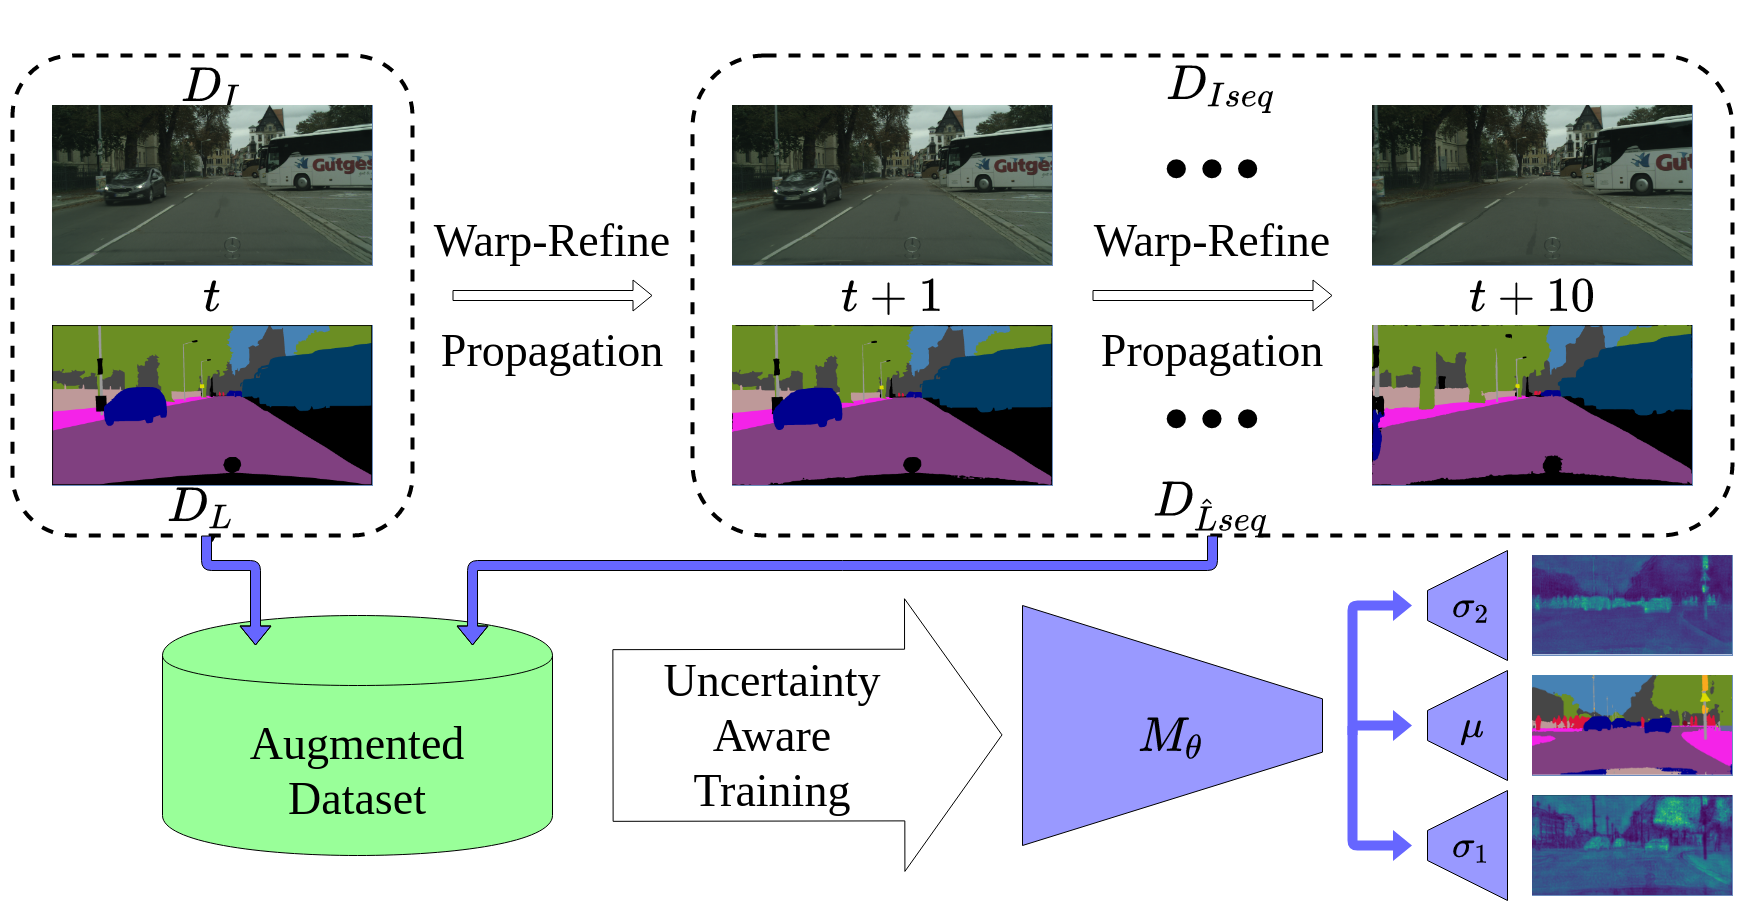
\includegraphics[clip,width=0.315\textwidth]{figures/fig_overview_lowres.png}%
% }
				\centering
				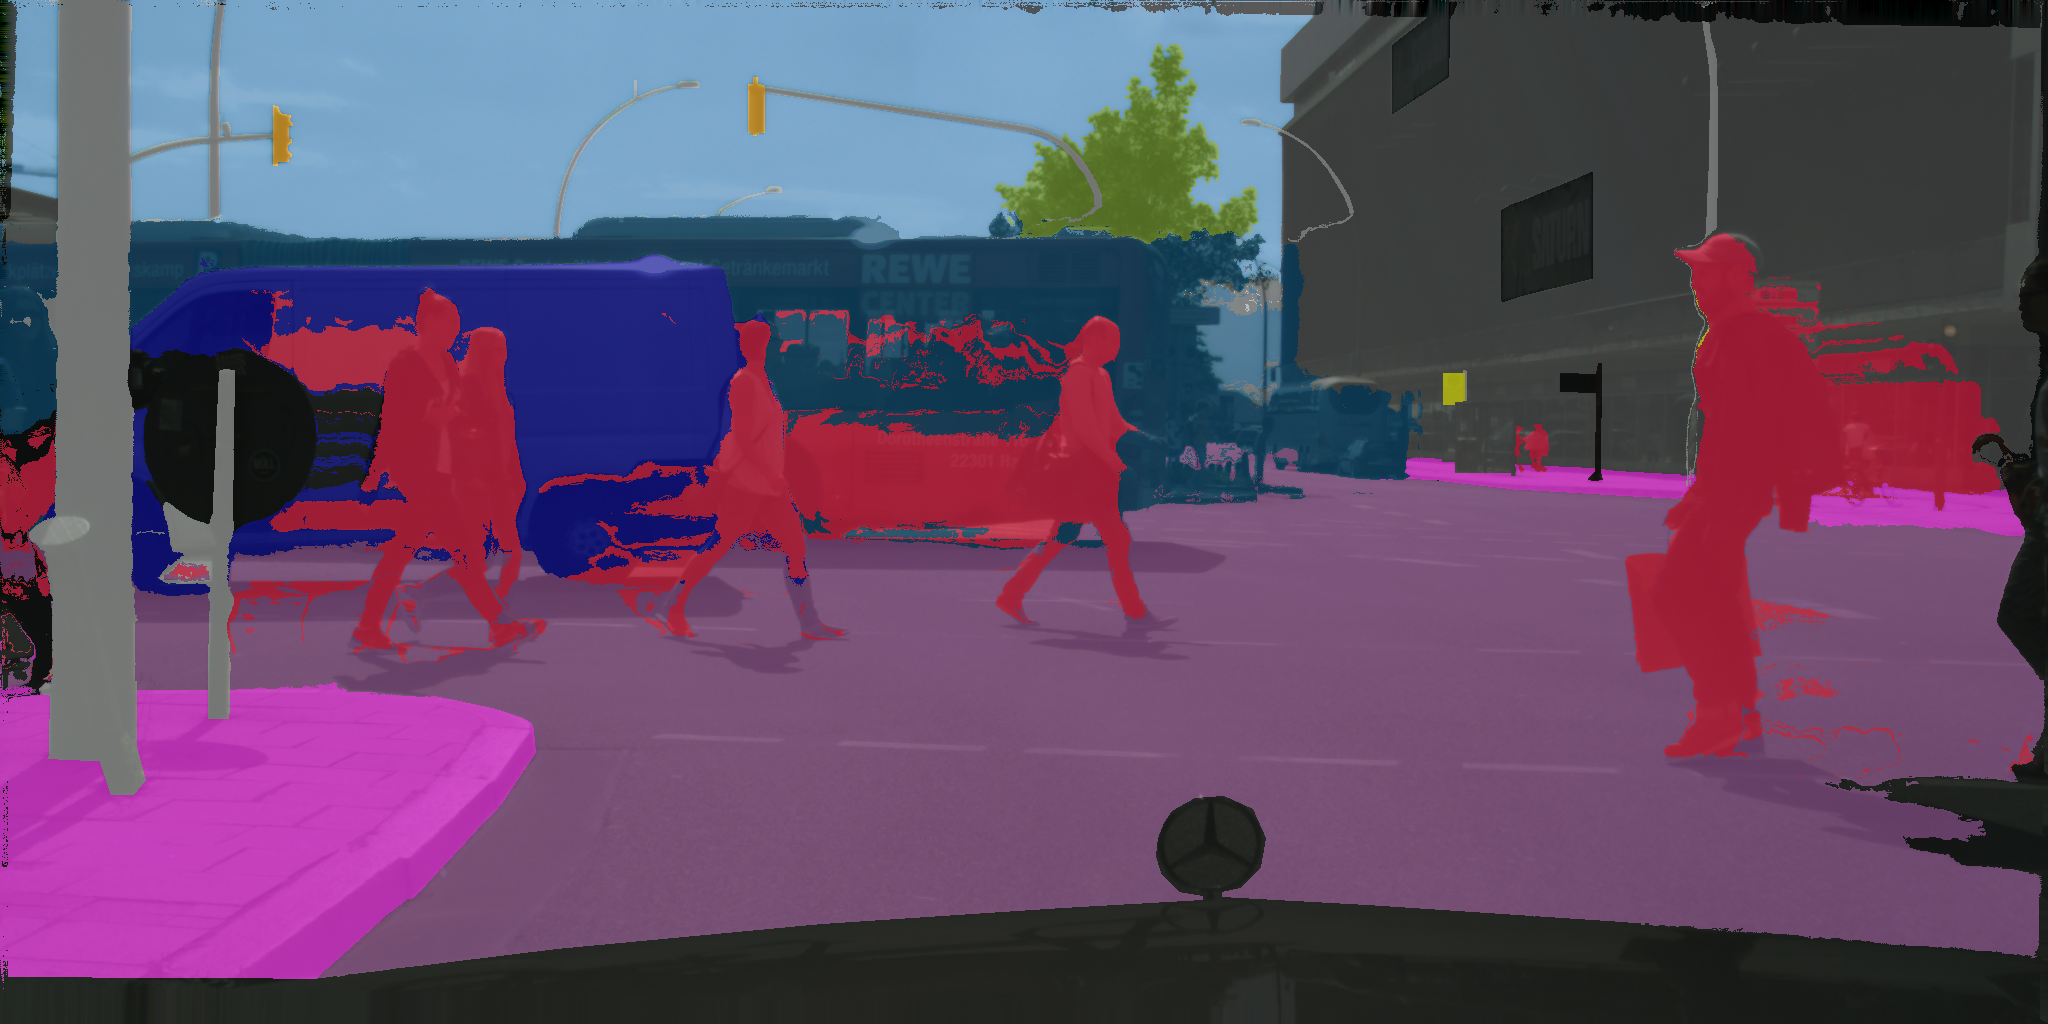
\includegraphics[width=\textwidth]{figures/prev_2.png}
				\vfill
				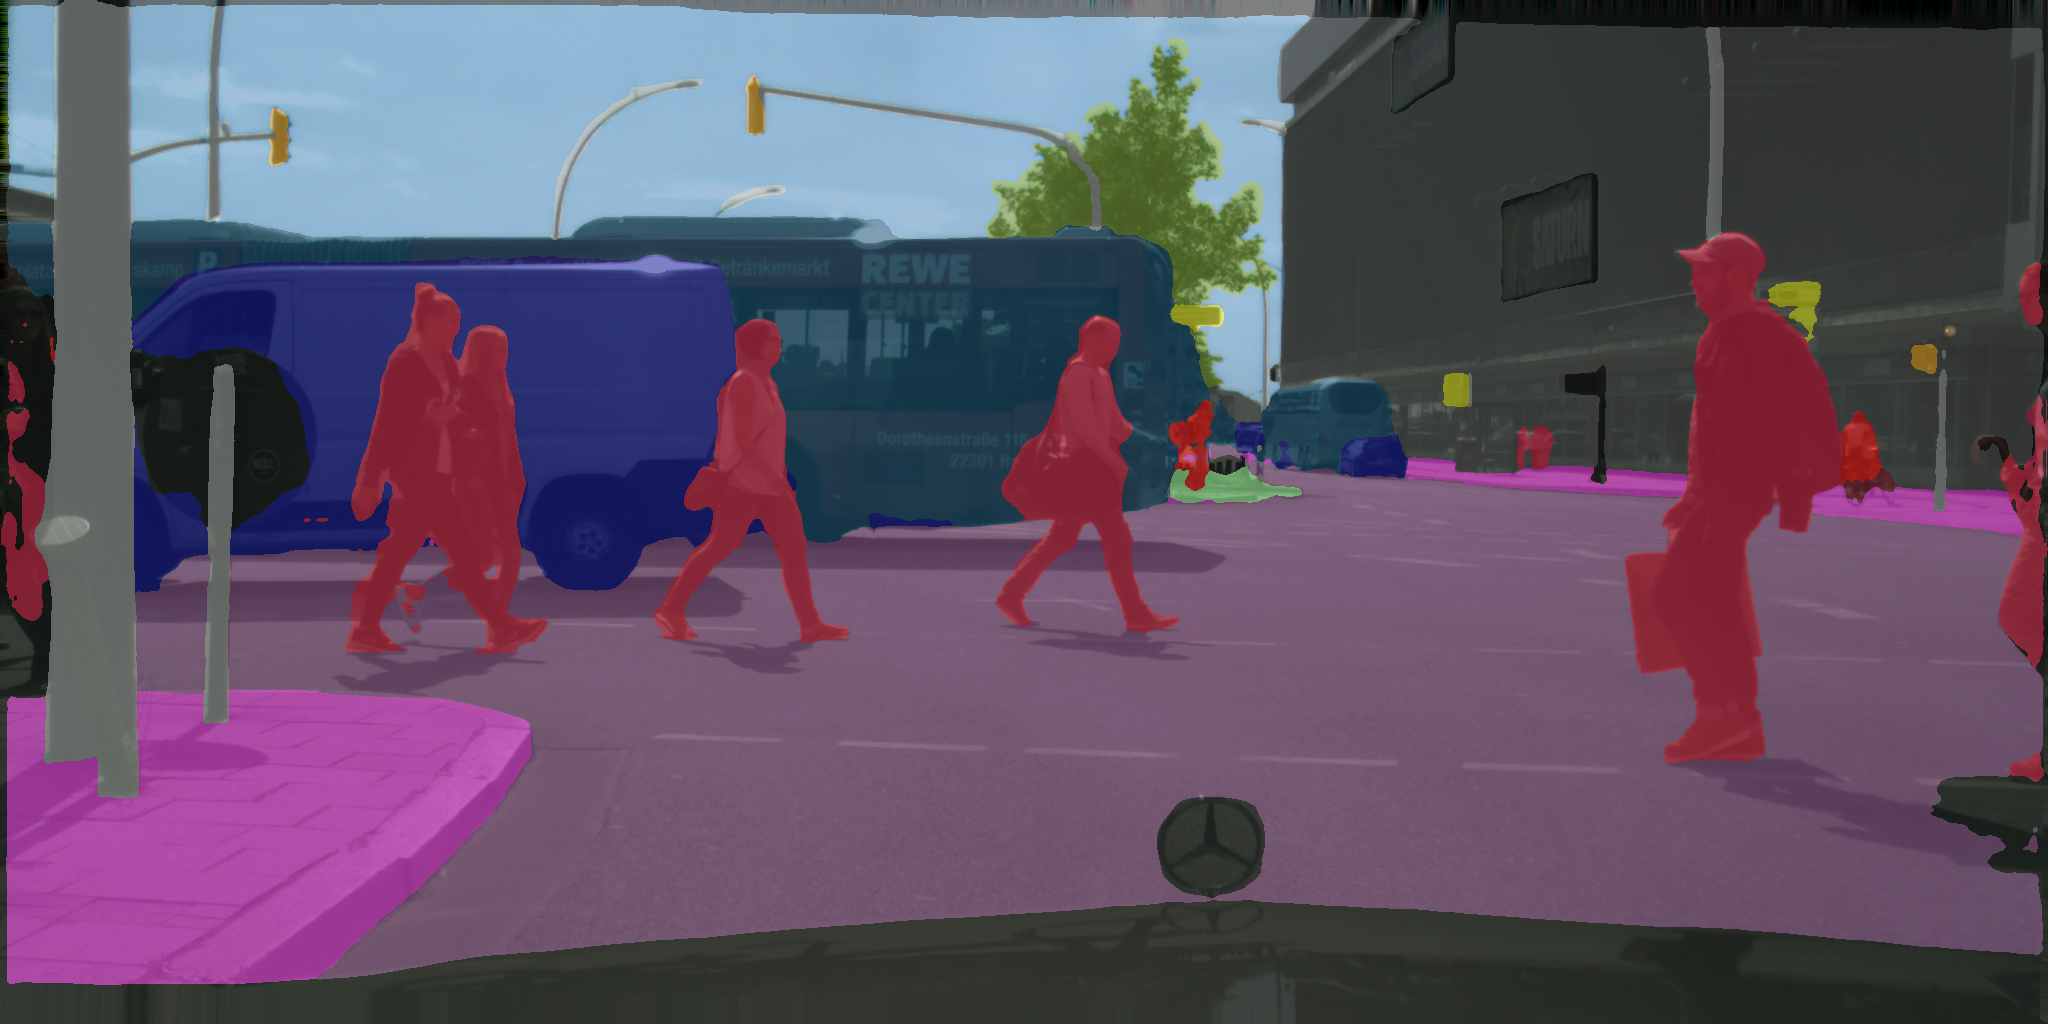
\includegraphics[width=\textwidth]{figures/our_2.png}%
				\vspace{0.3em}
			\end{minipage}
		}
    \vspace{-0.5em}
		\caption{\small (a) Using our propagation method, we generate pseudo-labels for images $D_{Iseq}$. The generated and the clean labels are then used for uncertainty-aware-training of semantic segmentation models. (b) Our method significantly surpasses \textit{state-of-the-art} label propagation methods~\cite{nvidia_cvpr19}.
		}
		\vspace{-0.5em}
	\end{figure}
